% ----------------------------------------------------------
% GESTÃO DE TEMPO / CRONOGRAMA
% ----------------------------------------------------------
\section{Cronograma}

A princípio temos uma organização dos macro-itens (Epics) que precisam ser desenvolvidos durante o projeto, dentro dos quais estipulamos as tarefas a serem feitas. Por meio do \gls{jira} podemos ter uma visão geral do andamento das Epics e os prazos, além das \glspl{sprint} planejadas e a atual.

\begin{figure}[H]
	\centering
	\caption{\label{jira-geral}Roteiro Geral}
	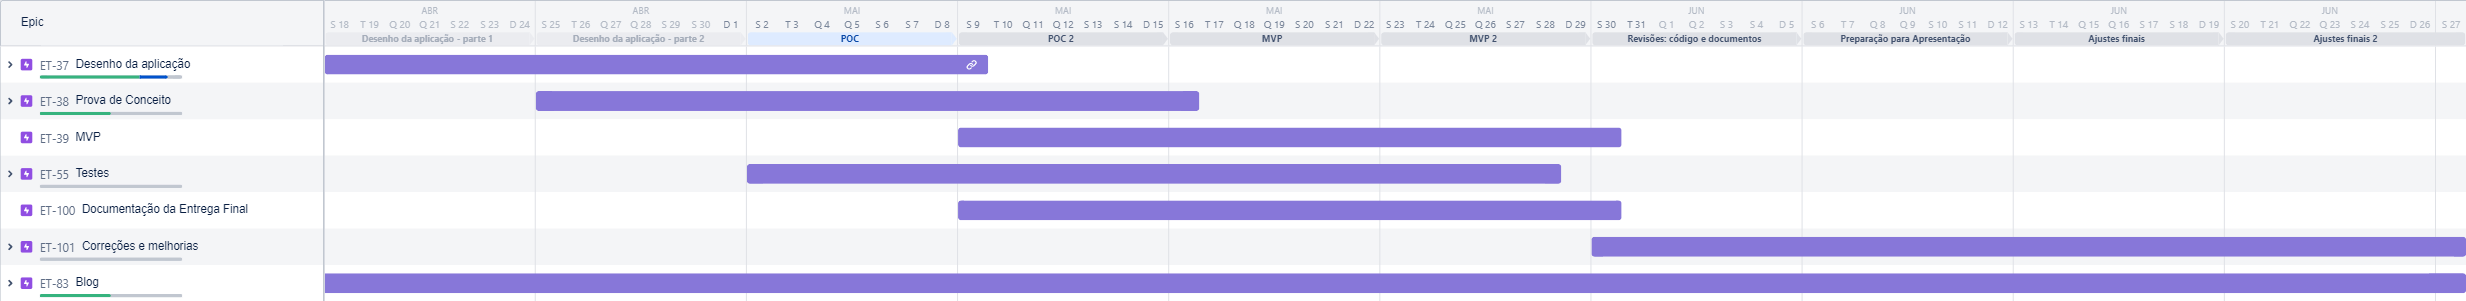
\includegraphics[width=0.95\textwidth]{imagens/cronograma-geral.png}
	\fonte{Roteiro via ferramenta \gls{jira}}
\end{figure}

\begin{figure}[H]
	\centering
	\caption{\label{jira-detalhe1}Roteiro Geral - Detalhe Inicial}
	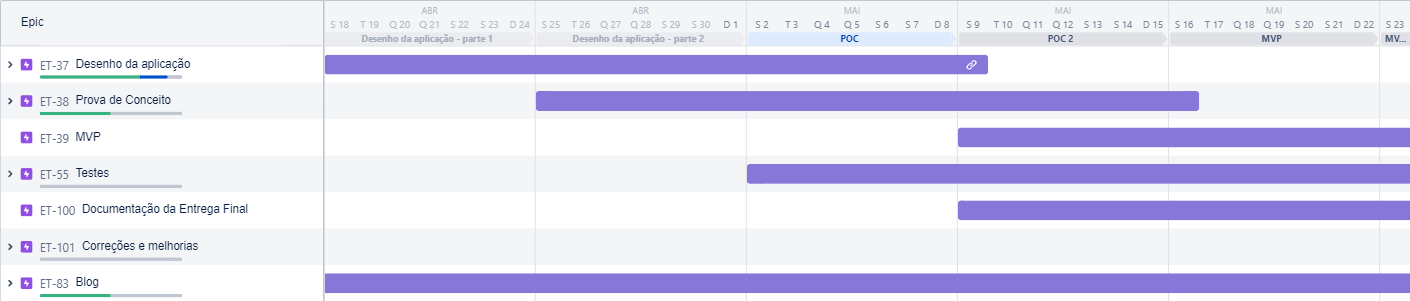
\includegraphics[width=0.95\textwidth]{imagens/cronograma-detalhe1.png}
	\fonte{Roteiro via ferramenta \gls{jira}}
\end{figure}

\begin{figure}[H]
	\centering
	\caption{\label{jira-detalhe2}Roteiro Geral - Detalhe Final}
	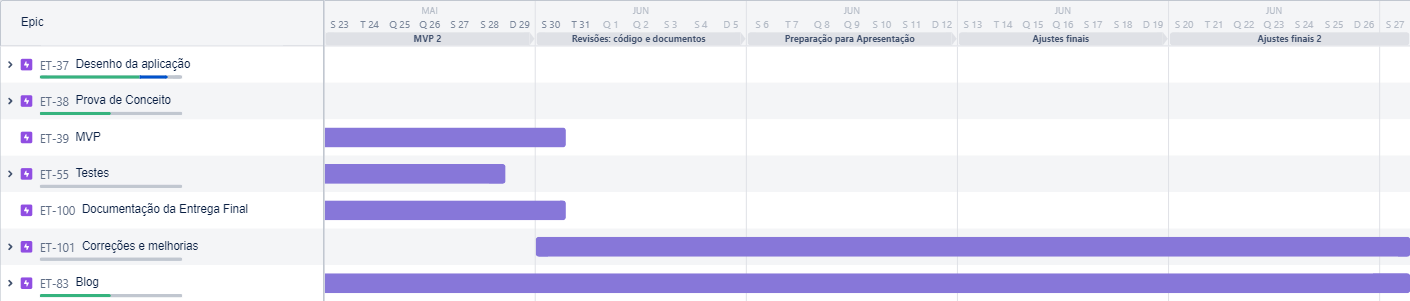
\includegraphics[width=0.95\textwidth]{imagens/cronograma-detalhe2.png}
	\fonte{Roteiro via ferramenta \gls{jira}}
\end{figure}

Apresentamos em \autoref{cronogramasem1} as \glspl{sprint} e algumas informações expostas em \autoref{jira-geral}, \autoref{jira-detalhe1} e \autoref{jira-detalhe2}.

\begin{quadro}[H]
	\caption{Cronograma de \glspl{sprint}}
	\centering
	\begin{tabular}{| p{0.17\linewidth}  | c | c | p{0.25\linewidth} | c |}
		\hline
		\thead[l]{Sprint} & \thead{Data Inicial} & \thead{Data Final} & \thead[l]{Descrição} & \thead{Status}\\
		\hline
		Desenho da aplicação 1 & 18/04/22 & 25/04/22 & Elaboração da documentação do Desenho da Aplicação. & Concluída\\
		\hline
		Desenho da aplicação 2 & 25/04/22 & 02/05/22 &  Continuação da elaboração do Desenho da Aplicação. Planejamento para a \ac{poc}. & Concluída\\
		\hline
		POC & 02/05/22 & 09/05/22 & Finalização do Desenho da Aplicação. Início do desenvolvimento dos itens da \ac{poc} & Em progresso \\
		\hline
		POC 2 & 09/05/22 & 16/05/22 & Continuação do desenvolvimento dos itens da \ac{poc}. & Não iniciada\\
		\hline
		MVP & 16/05/22 & 23/05/22 & Aproveitamento do que foi desenvolvido para a \ac{poc} com melhorias e ampliação conforme possível para o \ac{mvp}. & Não iniciada\\
		\hline
		MVP 2 & 23/05/22 & 30/05/22 & Continuação do trabalho no desenvolvimento do \ac{mvp}. & Não iniciada\\
		\hline
		Revisões: código e documentos & 30/05/22 & 06/06/22 &  Finalização e revisão tanto do desenvolvimento quanto da documentação. & Não iniciada\\
		\hline
		Preparação para a Apresentação & 06/06/22 & 13/06/22 &  Organização e planejamento da apresentação do projeto e sua documentação. & Não iniciada\\
		\hline
		Ajustes finais & 13/06/22 & 20/06/22 &  Ajustes a serem feitos para correção e/ou melhoria do projeto apresentado. & Não iniciada\\
		\hline
		Ajustes finais 2 & 20/06/22 & 27/06/22 &  Finalização dos ajustes finais para a entrega definitiva do projeto no semestre. & Não iniciada\\
		\hline
		
	\end{tabular}
	\fonte{Os Autores}
	\label{cronogramasem1}
\end{quadro}